\pdfminorversion=4 % for acroread
\documentclass[aspectratio=169,t,xcolor={usenames,dvipsnames}]{beamer}
%\documentclass[t,handout,xcolor={usenames,dvipsnames}]{beamer}
\usepackage{../beamerstyle}
\usepackage{dsfont}
\usepackage{bm}
\usepackage[english]{babel}
\usepackage[utf8]{inputenc}
\usepackage{graphicx}
\usepackage{algorithm}
\usepackage[ruled,vlined,algo2e,linesnumbered]{algorithm2e}
%\usepackage[boxed,vlined]{algorithm2e}
\usepackage{hyperref}
\usepackage{booktabs}
\usepackage{mathtools}

\usepackage{amsmath,amssymb}
\usepackage{listings}
\lstset{frame=lines,framesep=3pt,numbers=left,numberblanklines=false,basicstyle=\ttfamily\small}

\usepackage{subfig}
\usepackage{multicol}
%\usepackage{appendixnumberbeamer}
%
\usepackage{tcolorbox}

\usepackage{pgfplots}
\usepackage{tikz}
\usetikzlibrary{trees} 
\usetikzlibrary{shapes.geometric}
\usetikzlibrary{positioning,shapes,shadows,arrows,calc,mindmap}
\usetikzlibrary{positioning,fadings,through}
\usetikzlibrary{decorations.pathreplacing}
\usetikzlibrary{intersections}
\usetikzlibrary{positioning,fit,calc,shadows,backgrounds}
\pgfdeclarelayer{background}
\pgfdeclarelayer{foreground}
\pgfsetlayers{background,main,foreground}
\tikzstyle{activity}=[rectangle, draw=black, rounded corners, text centered, text width=8em]
\tikzstyle{data}=[rectangle, draw=black, text centered, text width=8em]
\tikzstyle{myarrow}=[->, thick, draw=black]

% Define the layers to draw the diagram
\pgfdeclarelayer{background}
\pgfdeclarelayer{foreground}
\pgfsetlayers{background,main,foreground}

%\usepackage{listings}
%\lstset{numbers=left,
%  showstringspaces=false,
%  frame={tb},
%  captionpos=b,
%  lineskip=0pt,
%  basicstyle=\ttfamily,
%%  extendedchars=true,
%  stepnumber=1,
%  numberstyle=\small,
%  xleftmargin=1em,
%  breaklines
%}

 
\definecolor{blue}{RGB}{0, 74, 153}

\usetheme{Boadilla}
%\useinnertheme{rectangles}
\usecolortheme{whale}
\setbeamercolor{alerted text}{fg=blue}
\useoutertheme{infolines}
\setbeamertemplate{navigation symbols}{\vspace{-5pt}} % to lower the logo
\setbeamercolor{date in head/foot}{bg=blue} % blue
\setbeamercolor{date in head/foot}{fg=white}
\setbeamercolor{author in head/foot}{bg=blue} %blue
\setbeamercolor{title in head/foot}{bg=blue} % blue
\setbeamercolor{title}{fg=white, bg=blue}
\setbeamercolor{block title}{fg=white,bg=blue}
\setbeamercolor{block body}{bg=blue!10}
\setbeamercolor{frametitle}{fg=white, bg=blue}
\setbeamercovered{invisible}

\makeatletter
\setbeamertemplate{footline}
{
  \leavevmode%
  \hbox{%
  \begin{beamercolorbox}[wd=.333333\paperwidth,ht=2.25ex,dp=1ex,center]{author in head/foot}%
    \usebeamerfont{author in head/foot}\insertshortauthor
  \end{beamercolorbox}%
  \begin{beamercolorbox}[wd=.333333\paperwidth,ht=2.25ex,dp=1ex,center]{title in head/foot}%
    \usebeamerfont{title in head/foot}\insertshorttitle
  \end{beamercolorbox}%
  \begin{beamercolorbox}[wd=.333333\paperwidth,ht=2.25ex,dp=1ex,right]{date in head/foot}%
    \usebeamerfont{date in head/foot}Week \@week, Topic \@topicnumber, Slide \insertframenumber{}\hspace*{2em}
%    \insertframenumber\hspace*{2ex} 
  \end{beamercolorbox}}%
  \vskip0pt%
}

\newcommand{\@week}{0}
\newcommand{\@topicnumber}{0}
\newcommand{\week}[1]{\renewcommand{\@week}{#1}}
\newcommand{\topicnumber}[1]{\renewcommand{\@topicnumber}{#1}}

\makeatother

%\pgfdeclareimage[height=1.2cm]{automl}{images/logos/automl.png}
%\pgfdeclareimage[height=1.2cm]{freiburg}{images/logos/freiburg}

%\logo{\pgfuseimage{freiburg}}

\input{../latex_main/macros}




\newcommand{\inducer}{\mathcal{I}}
\newcommand{\R}{\mathds{R}}

%The following might look confusing but allows us to switch the notation of the optimization problem independently from the notation of the hyper parameter optimization
\newcommand{\xx}{\conf} %x of the optimizer
\newcommand{\xxi}[1][i]{\conf_{#1}} %i-th component of xx (not confuse with i-th individual)
\newcommand{\XX}{\pcs} %search space / domain of f
\newcommand{\f}{\cost} %objective function

\newenvironment{blocki}[1] % itemize block
{
 \begin{block}{#1}\begin{itemize}
}
{
\end{itemize}\end{block}
}

\title[AutoML: Hyperparameter Optimization]{AutoML: Hyperparameter Optimization}
%\subtitle{Overview for this Week} %To be defined in source!
%TODO: change authors!
\author[Jakob Richter]{Bernd Bischl \and Frank Hutter \and Lars Kotthoff\newline \and Marius Lindauer}
\institute{}
\date{}

\subtitle{Evolutionary Algorithms}
\week{4}
\topicnumber{3}


\begin{document}

\maketitle


%----------------------------------------------------------------------
%----------------------------------------------------------------------

\begin{frame}[containsverbatim]{Evolutionary algorithms}

\textbf{Evolutionary algorithms} (EA) are a class of stochastic, metaheuristic optimization techniques whose mode of operation is inspired by the evolution of natural organisms.

\vspace{0.5cm}

History of evolutionary algorithms:

\begin{itemize}
\item \textbf{Genetic algorithms}: Use binary problem representation, therefore closest to the biological model of evolution.
\item \textbf{Evolution strategies}: Use direct problem representation, e.g., vector of real numbers.
\item \textbf{Genetic programming}: Create structures that convert an input into a fixed output (e.g. computer programs); solution candidates are represented as trees.
\item \textbf{Evolutionary programming}: Similar to GP, but solution candidates are not represented by trees, but by finite state machines.
\end{itemize}

The boundaries between the terms become increasingly blurred and are often used synonymously.
\end{frame}

\begin{frame}{Structure of an evolutionary algorithm}
\begin{center}
\begin{figure}
\centering
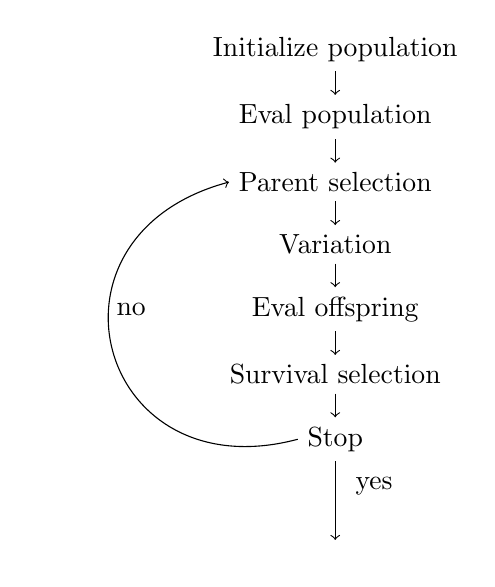
\begin{tikzpicture}[node distance=0.8cm, auto,]
%nodes
\node (init) {Initialize population};
\node[below = 0.3cm of init](rating1) {Eval population};
\node[below = 0.3cm of rating1](selection1) {Parent selection};
\node[below = 0.3cm of selection1](variation) {Variation};
\node[below = 0.3cm of variation](rating2) {Eval offspring};
\node[below = 0.3cm of rating2](selection2) {Survival selection};
\node[below = 0.3cm of selection2](stop) {Stop};
\node[below = 1cm of stop](dummy2) {};
\node[below = 0.2cm of stop](dummy3) {};
\node[right = 0.01cm of dummy3](dummy4) {yes};
\node[left = 1.1cm of rating2](dummy1) {no};
\draw[->] (init) to (rating1) node[midway, above]{};
\draw[->] (rating1) to (selection1) node[midway, above]{};
\draw[->] (selection1) to (variation) node[midway, above]{};
\draw[->] (variation) to (rating2) node[midway, above]{};
\draw[->] (rating2) to (selection2) node[midway, above]{};
\draw[->] (selection2) to (stop) node[midway, above]{};
\draw[->] (stop) to (dummy2) node[midway, above]{};
\draw[->] (stop) to [bend left=90, looseness=2](selection1) node[midway, above]{};
\end{tikzpicture}
\end{figure}
\end{center}

\end{frame}


\begin{frame}{Notation and Terminology}
\begin{center}
\begin{tabular}{ c | c }
\textbf{Symbols} & \textbf{EA Terminology} \\
\hline \\
Solution candidate $\xx \in \XX$ & Chromosome of an individual \\
$\xxi$& $i$-th gene of chromosome\\
Set of candidates $\mathcal{P}$ with $\mu = |\mathcal{P}|$ & Population and size\\
$\lambda$ & Number of generated offsprings\\
$\f: \XX \to \R$ & Fitness function
\end{tabular}
\end{center}

$$\f(\xx) = \widehat{GE}_{\datasettest}\left(\inducer(\datasettrain, \xx)\right)$$

Notation clash:
\begin{itemize}
    \item In EAs the objective function is often denoted $f(x)$.
    \item As these symbols are used for ML already we use $\cost(\conf)$ and $\conf$ instead of $f$ and $x$.
    \item Be careful: The offspring size $\lambda$ is different from the candidate $\xx$ (bold symbol!).
\end{itemize}
\end{frame}


\begin{frame}{Step 1: Initialize population}
    \begin{itemize}
            \item A evolutionary algorithm is started by generating a initial population $\mathcal{P} = \{\xx^{(1)}, ..., \xx^{(\mu)}\}$.
            \item Usually we sample this uniformly at random.
            \item We could introduce problem prior knowledge via a smarter init procedure.
            \item This population is evaluated, i.e., the objective function is computed for every individual in the initial population.
            \item The initialization can have a large influence on the quality of the found solution, so many EAs employ \textit{restarts} with new randomly generated populations.
    \end{itemize}

\end{frame}

\begin{frame}[containsverbatim,allowframebreaks]{Step 2: Parent selection}


In the first step of an iteration, $\lambda$ parents are chosen, who create offspring in the next step.


\begin{columns}
\begin{column}{0.5\textwidth}

  Possibilities for selection of parents:

  \begin{itemize}
    \item \textbf{Neutral selection: }choose individual with a probability $1/\mu$.
    \item \textbf{Fitness-proportional selection: }draw individuals with probability proportional to their fitness.
  \end{itemize}
\end{column}%
\begin{column}{0.5\textwidth}
  \begin{itemize}
    \item \textbf{Tournament Selection: }randomly select $k$ individuals for a "Tournament Group". Of the drawn individuals, the best one (with the highest fitness value) is then chosen. Procedure is performed $\lambda$-times.
  \end{itemize}

  \begin{figure}
    \includegraphics[width = 0.9\linewidth]{images/tournament_selection_c.pdf}
  \end{figure}

\end{column}
\end{columns}

\end{frame}

\begin{frame}{Step 3: Variation}

New individuals are now generated from the parent population. This is done by

\begin{itemize}
\item Recombination/Crossover: combine two parents into one offspring.
\item Mutation: (locally) change an individual.
\end{itemize}

Sometimes only one operation is performed.

\end{frame}

\begin{frame}{Recombination for numeric representations}

Two individuals $\xx, \tilde\xx \in \R^n$ in numerical representation can be recombined as follows:

\begin{itemize}
\item \textbf{Uniform crossover}: choose gene $i$ with probability $p$ of 1st parent and probability $1-p$ of 2nd parent.
\item \textbf{Intermediate recombination}: new individual is created from the mean value of two parents $\frac{1}{2}(\xx + \tilde\xx)$
\item \textbf{Simulated Binary Crossover (SBX)}: generate \textbf{two offspring} based on

$$
\bar\xx \pm \frac{1}{2} \beta (\tilde\xx - \xx)
$$

with $\bar\xx = \frac{1}{2} (\xx + \tilde\xx)$ and $\beta$ randomly sampled from a certain distribution.
\end{itemize}

\end{frame}

\begin{frame}[containsverbatim]{Mutation for numeric representations \litw{{\href{https://www.researchgate.net/publication/262320509_Analysing_mutation_schemes_for_real-parameter_genetic_algorithms}{K. Deb and D. Deb. 2014}}}}
  \textbf{Mutation:} individuals are changed, for example for $\xx \in \R^n$
  \begin{itemize}
  \item \textbf{Uniform mutation:} choose a random gene $\xxi$ and replace it with a value uniformly distributed (within the feasible range).
  \item \textbf{Gauss mutation}: $\tilde\xx = \xx \pm \sigma \mathcal{N}(0, \boldsymbol{I})$
  \item \textbf{Polynomial mutation:} polynomial distribution instead of normal distribution
  \begin{center}
  \begin{figure}
    \includegraphics[height = 3.5cm, width = 4cm]{images/polynomial_mutation.png}\\
      %\scriptsize{Source: K. Deb, Analysing mutation schemes for real-parameter genetic algorithms, 2014}
  \end{figure}
   \end{center}
   % \framebreak
  % More exact:
  % $$
  % {\tilde \xxi} = \xxi + (\xxi[i,\text{upper}] - \xxi[i,\text{lower}]) \delta_{i}
  % $$
  % with $\xxi[i,\text{upper}]$ ($\xxi[i,\text{lower}]$) as upper (lower) bound for $\xxi$.
  % $\delta_{i}$ results as:
  % \footnotesize
  % $$
  % \delta_{i} =
  % \begin{cases}
  % [2r_{i}+(1-2r_{i})(1-\delta)^{\eta_{m}+1}]^{\frac{1}{\eta +1}} -1, & r_{i} < 0.5 \\
  % 1 - [2(1-r_{i})+2(r_{i}-\frac{1}{2})(1-\delta)^{\eta_{m}+1}]^{\frac{1}{\eta_{m} +1}}, &  \text{else.}
  % \end{cases}
  % $$
  % with  $\delta = \frac{min\{(x_{i} - \xxi[i,\text{upper}]), (\xxi[i,\text{upper}]-\xxi)\}}{\xxi[i,\text{upper}] - \xxi[i,\text{upper}]}$.
  % \normalsize
  % \vspace{0.5cm}
  % Here $r_{i} \in [0,1]$ is a uniformly distributed number, $\eta_{m}$ is the distribution index of the mutation and is chosen by the user.\\
  % % Remark: A $\eta_{m}$ of the order of $\eta_{m} \in [20,100]$ is common.
  % \normalsize
  \end{itemize}
  % \vspace{0.5cm}

  \end{frame}

\begin{frame}{Recombination for bit strings}

  Two individuals $\xx, \tilde\xx \in \{0, 1\}^n$ encoded as bit strings can be recombined as follows:

  \begin{itemize}
  \item \textbf{1-point crossover}: select crossover $k \in \{1, ..., n - 1\}$ randomly and select the first $k$ bits from 1st parent, the last $n-k$ bits from 2nd parent.

  \footnotesize
  \begin{center}
  \begin{tabular}{c @{\hspace{2\tabcolsep}} *{6}{c}}
      \textcolor{red}{1} & \textcolor{blue}{1}  & & \textcolor{red}{1}  \\
      \textcolor{red}{0} & \textcolor{blue}{0}  & &  \textcolor{red}{0}  \\ \cmidrule{1-4}
    \textcolor{red}{0} & \textcolor{blue}{1}  &$\Rightarrow$ & \textcolor{blue}{1}  \\
    \textcolor{red}{1} & \textcolor{blue}{1}  & &   \textcolor{blue}{1}  \\
    \textcolor{red}{1} & \textcolor{blue}{0}  & &   \textcolor{blue}{0}
  \end{tabular}
  \end{center}
  \normalsize

  \item \textbf{Uniform crossover}: select bit $i$ with probability $p$ of 1st parent and $1-p$ of 2nd parent.
  
      \footnotesize
  \begin{center}
  \begin{tabular}{c @{\hspace{2\tabcolsep}} *{6}{c}}
      \textcolor{red}{1} & \textcolor{blue}{0}  & & \textcolor{red}{1}  \\
      \textcolor{red}{0} & \textcolor{blue}{0}  & &  \textcolor{blue}{0}  \\ 
    \textcolor{red}{0} & \textcolor{blue}{1}  &$\Rightarrow$ & \textcolor{blue}{1}  \\
    \textcolor{red}{0} & \textcolor{blue}{1}  & &   \textcolor{blue}{1}  \\
    \textcolor{red}{1} & \textcolor{blue}{0}  & &   \textcolor{red}{1}
  \end{tabular}
  \end{center}
  \normalsize

  \end{itemize}


  % \footnotesize
  % \begin{center}
  % \begin{tabular}{c @{\hspace{2\tabcolsep}} *{6}{c}}
  %  " " & \textcolor{red}{1} & \textcolor{blue}{1} & " " & " " & "  " & \textcolor{red}{1}  \\
  %  " " & \textcolor{red}{0} & \textcolor{blue}{0} & " " & " " & "  " & \textcolor{blue}{0}  \\
  %  " " & \textcolor{red}{0} & \textcolor{blue}{1} & " " &$\Rightarrow$ & "  " & \textcolor{blue}{1}  \\
  %  " " & \textcolor{red}{1} & \textcolor{blue}{1} & " " & " " & "  " & \textcolor{blue}{1}  \\
  %  " " & \textcolor{red}{1} & \textcolor{blue}{0} & " " & " " & "  " & \textcolor{red}{1}
  % \end{tabular}
  % \end{center}
  % \normalsize

  \end{frame}

  \begin{frame}{Mutation for bit strings}
  An individual $\xx \in \{0, 1\}^n$ encoded as a bit string can be mutated as follows:
  \vspace{0.5cm}
  % \textbf{Mutation:}
  \begin{itemize}
  \item \textbf{Bitflip}: for each index $k \in \{1, ..., n\}$: bit $k$ is flipped with probability $p \in (0,1)$.
  \end{itemize}
  \begin{center}
  \begin{tabular}{c @{\hspace{2\tabcolsep}} *{5}{c}}
  \\[1ex]
   1  &               & \textcolor{red}{0}  \\
   0  &               & 0  \\
   0  & $\Rightarrow$ & 0  \\
   0  &               & \textcolor{red}{1}  \\
   1  &               & 1
  \end{tabular}
  \end{center}
  \end{frame}
  \begin{frame}{Step 4: Survival selection}
  Now individuals are chosen who survive. Two common strategies are:
  \begin{itemize}
  \item \textbf{$(\mu, \lambda)$-selection}: we select from the $\lambda$ descendants the $\mu$ best ($\lambda \ge \mu$ necessary).
  \textbf{But:} best overall individual can get lost!
  \item \textbf{$(\mu + \lambda)$-selection}: $\mu$ parents and $\lambda$ offspring are lumped together and the $\mu$ best individuals are chosen.
  Best individual safely survives.
  \end{itemize}

\end{frame}


\begin{frame}[allowframebreaks]{Example of an evolutionary algorithm}

    In the following, a (simple) EA is shown on the 1-dim Ackley function, optimized on $[-30, 30]$.

\vspace{0.5cm}

Usually for the optimization of a function $\f:\R^n \to \R$ individuals are coded as real vectors $\xx \in \R^n$, so here we use simply one real number as chromosome.

\begin{center}
\begin{figure}
\includegraphics[height=4cm]{images/ea_ex1.png}
\end{figure}
\end{center}

\framebreak
Randomly init population with size $\mu = 20$.

\begin{center}
\begin{figure}
\includegraphics[height=6cm]{images/ea_ex2.png}
\end{figure}
\end{center}


\framebreak

We choose $\lambda = 5$ offspring by neutral selection (red individuals).

\begin{center}
\begin{figure}
\includegraphics[height=6cm]{images/ea_ex3.png}
\end{figure}
\end{center}

\framebreak

We use a Gauss mutation with $\sigma = 2$ and do not apply a recombination.
 \begin{center}
    \begin{figure}
    \includegraphics[height=6cm]{images/ea_ex4.png}
    \end{figure}
    \end{center}

  \framebreak

We use a $(\mu + \lambda)$ selection. The selected individuals are green.

  \begin{center}
    \begin{figure}
      \includegraphics[height=6cm]{images/ea_ex5.png}
    \end{figure}
  \end{center}


\end{frame}


\begin{frame}{Evolutionary Algorithms}

  \begin{blocki}{Advantages}
    \item Conceptually simple, yet powerful enough to solve complex problems (including HPO)
    \item All parameter types possible in general
    \item Highly parallelizable (depends on $\lambda$)
    \item Allows customization via specific variation operators
    \end{blocki}

    \begin{blocki}{Disadvantages}
      \item Less theory available (for realistic, complex EAs)
    \item Can be hard to get balance between exploration and exploitation right
        \item Can have quite a few control parameters, hard to set them correctly\\
        \item Customization necessary for complex problems
        \item Not perfectly suited for expensive problems like HPO, 
            as quite a higher number of evaluations is usually
            needed for appropriate convergence / progress
    % \item Stagnation: Optimization process does not progress any more %FIXME: JR: Isn't that the same as the point below?
    % \item Premature Convergence: Algorithm converges to a single solution, which is not as good as expected
    % \item Diversity of population structures: Loss of population diversity for solving complex optimization problems
    \end{blocki}

\end{frame}

% \begin{frame}{More Tuning Algorithms}

% There are many more methods for hyperparmeter tuning, some of which will be discussed in later parts of this lecture:


% \begin{itemize}
% \item Stochastic local search, e.g. simulated annealing
% \item Bayesian optimization
% \item Hyperband
% \item Iterated F-Racing
% \item many more $\dots$
% \end{itemize}

% \end{frame}

\end{document}
